%%%%%%%%%%%%%%%%%%%%%%%%%%%%%%%%%%%%%%%%%
% Jacobs Landscape Poster
% LaTeX Template
% Version 1.0 (29/03/13)
%

% 

% This template has been downloaded from:
% http://www.LaTeXTemplates.com
%
%%%%%%%%%%%%%%%%%%%%%%%%%%%%%%%%%%%%%%%%%

%----------------------------------------------------------------------------------------
%	PACKAGES AND OTHER DOCUMENT CONFIGURATIONS
%----------------------------------------------------------------------------------------

\documentclass[final]{beamer}
\usepackage[center]{caption}

\usepackage[scale=1.24]{beamerposter} % Use the beamerposter package for laying out the poster
\usepackage{graphicx}
\usepackage{array}
\usepackage{tabu}

\usetheme{confposter} % Use the confposter theme supplied with this template

\setbeamercolor{block title}{fg=blue,bg=white} % Colors of the block titles
\setbeamercolor{block body}{fg=black,bg=white} % Colors of the body of blocks
\setbeamercolor{block alerted title}{fg=white,bg=blue!70} % Colors of the highlighted block titles
\setbeamercolor{block alerted body}{fg=black,bg=dblue!10} % Colors of the body of highlighted blocks
% Many more colors are available for use in beamerthemeconfposter.sty

%-----------------------------------------------------------
% Define the column widths and overall poster size
% To set effective sepwid, onecolwid and twocolwid values, first choose how many columns you want and how much separation you want between columns
% In this template, the separation width chosen is 0.024 of the paper width and a 4-column layout
% onecolwid should therefore be (1-(# of columns+1)*sepwid)/# of columns e.g. (1-(4+1)*0.024)/4 = 0.22
% Set twocolwid to be (2*onecolwid)+sepwid = 0.464
% Set threecolwid to be (3*onecolwid)+2*sepwid = 0.708

\newlength{\sepwid}
\newlength{\onecolwid}
\newlength{\twocolwid}
\newlength{\threecolwid}
\setlength{\paperwidth}{48in} % A0 width: 46.8in
\setlength{\paperheight}{36in} % A0 height: 33.1in
\setlength{\sepwid}{0.024\paperwidth} % Separation width (white space) between columns
\setlength{\onecolwid}{0.22\paperwidth} % Width of one column
\setlength{\twocolwid}{0.464\paperwidth} % Width of two columns
\setlength{\threecolwid}{0.708\paperwidth} % Width of three columns
\setlength{\topmargin}{-0.5in} % Reduce the top margin size
%-----------------------------------------------------------

\usepackage{graphicx}  % Required for including images
\usepackage{biblatex}
\usepackage{booktabs} % Top and bottom rules for tables

%----------------------------------------------------------------------------------------
%	TITLE SECTION 
%----------------------------------------------------------------------------------------

\title{Fairness in Diffusion Models} % Poster title

\author{{\huge David Yang}} % Author(s)

\institute{{ Project in collaboration with Amy Feng, Alexander Goslin, and Selena She @ REU-CAAR (University of Maryland, College Park).}} % Institution(s)

%----------------------------------------------------------------------------------------

\addbibresource{sample.bib}
\begin{document}

\addtobeamertemplate{block end}{}{\vspace*{2ex}} % White space under blocks
\addtobeamertemplate{block alerted end}{}{\vspace*{2ex}} % White space under highlighted (alert) blocks

\setlength{\belowcaptionskip}{1ex} % White space under figures
\setlength\belowdisplayshortskip{2ex} % White space under equations

\begin{frame}[t] % The whole poster is enclosed in one beamer frame

\begin{columns}[t] % The whole poster consists of three major columns, the second of which is split into two columns twice - the [t] option aligns each column's content to the top

\begin{column}{\sepwid}\end{column} % Empty spacer column
\begin{column}{\onecolwid} % The first column

%----------------------------------------------------------------------------------------
%	OBJECTIVES
%----------------------------------------------------------------------------------------

\begin{alertblock}{Abstract}
	\begin{itemize}
	\item Generative Artificial Intelligence models have quickly grown in popularity, and their use has become very widespread. One such model, a diffusion model, generates an image for a given text prompt. Since these models are trained on large-scale datasets, they inherit many biases implicit in this data, thereby enforcing societal stereotypes. 
        \item In this project, we focus on images of people generated by Stable Diffusion. We aim to address gender and race stereotypes by modifying the image output of these diffusion models to yield a more fair and general representation of people of all genders and races.
	\end{itemize}
\end{alertblock}

%----------------------------------------------------------------------------------------
%	INTRODUCTION
%----------------------------------------------------------------------------------------

\begin{block}{Motivation}
\begin{itemize}
\item Generative AI such as Diffusion Models suffer from implicit biases (gender, race, age stereotypes).

\item Previous work such as \textsc{FairDiffusion} focuses on individual fairness, as the most commonly used large face dataset, FairFace, contains just single-person images.

\begin{center}
\begin{figure}
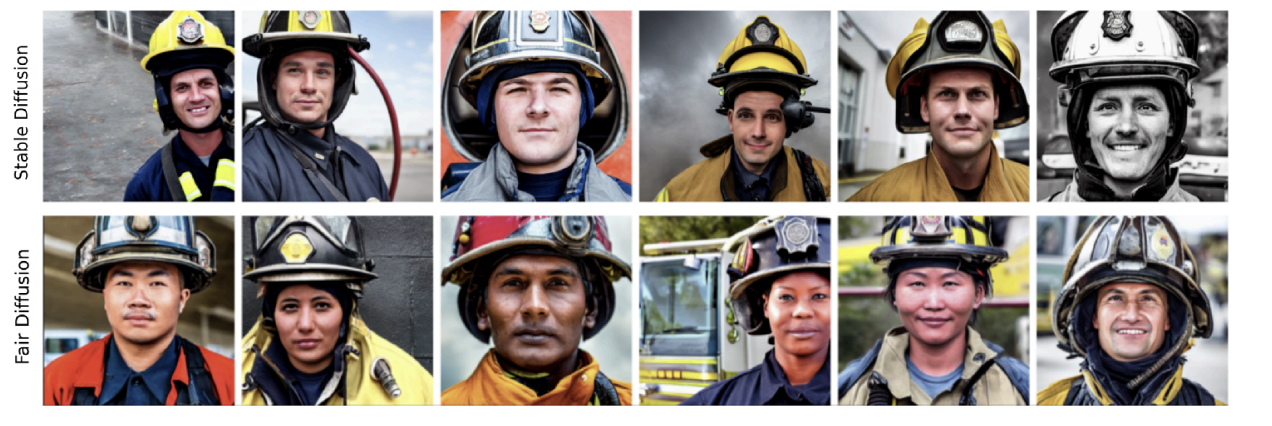
\includegraphics[scale=1.25]{FairDiffusionFirefighterOutput.png}
\captionsetup{justification=centering}
\caption{A previous approach, \textsc{FairDiffusion} \cite{friedrich2023fair}, handles individual images well, using \textsc{Sega} \cite{brack2023sega}.}
\end{figure}
\end{center}

\vspace{-1cm}

\item We are interested in improving fairness in diffusion models and extending previous work to solve fairness in group images.
\end{itemize}    
\end{block}

\begin{block}{Acknowledgments}
Thank you to my mentor Furong Huang and the REU-CAAR Program for making this research possible.
\end{block}

%------------------------------------------------



%----------------------------------------------------------------------------------------

\end{column} % End of the first column

% \begin{column}{0.02\linewidth} % Adjust the width as needed
%     \vrule % Add a vertical line here
%    \end{column}
\begin{column}{\sepwid}\end{column} % Empty spacer column

\begin{column}{\twocolwid} % Begin a column which is two columns wide (column 2)

\begin{columns}[t,totalwidth=\twocolwid] % Split up the two columns wide column

\begin{column}{\twocolwid}\vspace{-.6in} % The first column within column 2 (column 2.1)

%----------------------------------------------------------------------------------------
%	MATERIALS
%----------------------------------------------------------------------------------------



\begin{block}{General Pipeline}
    \begin{figure}
    %\centering
    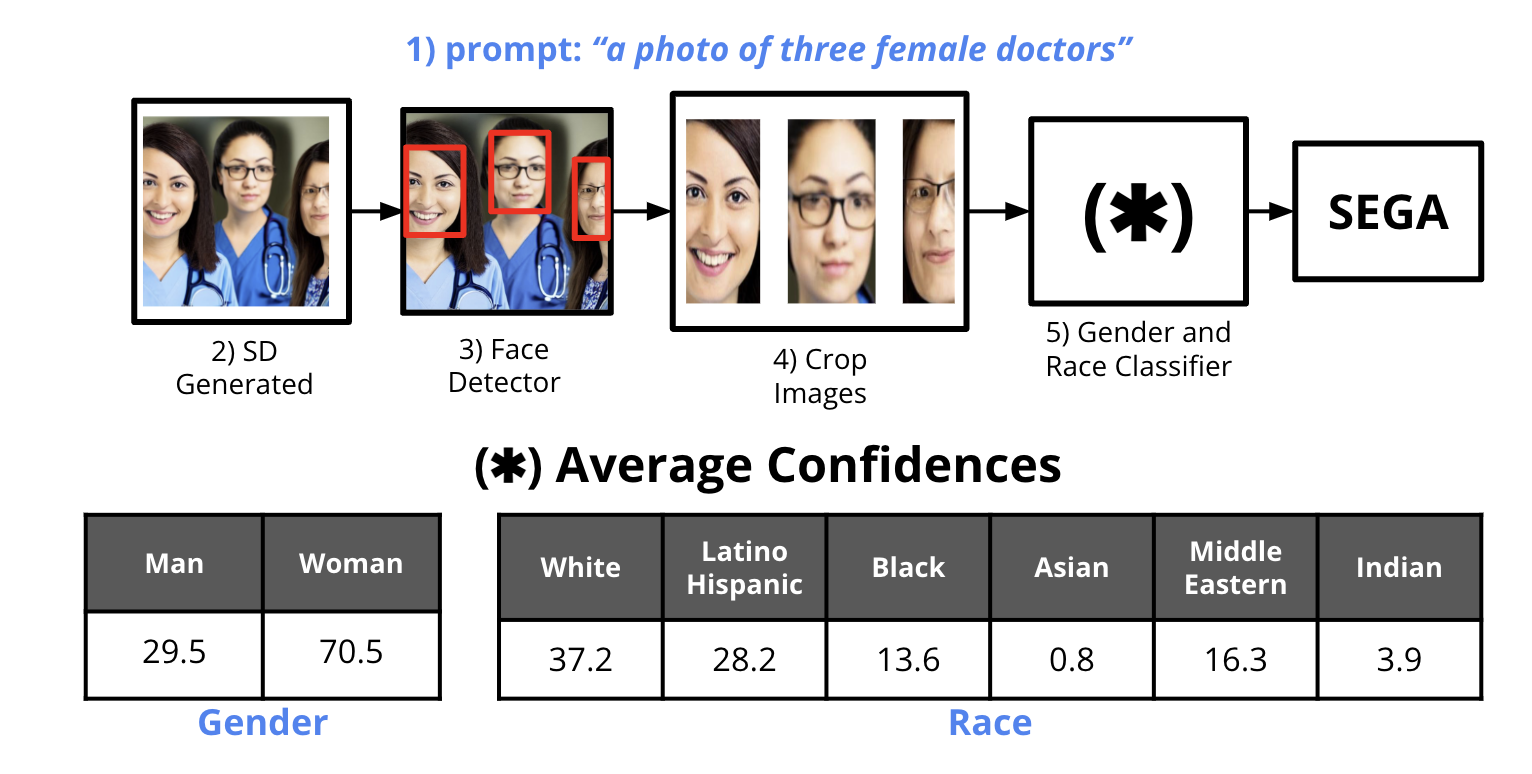
\includegraphics[scale = 1.35]{GeneralPipeline1.png}
    \end{figure}

\end{block}
\vspace{-1cm}
\begin{block}{Results (Individual Images)}
    \begin{figure}
    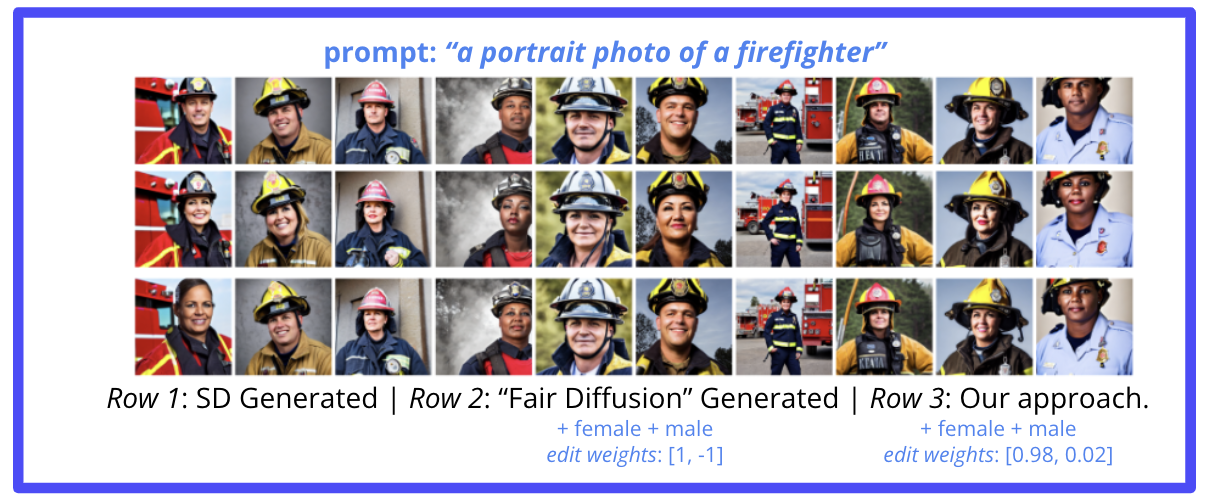
\includegraphics[scale = 1.7]{IndividualFairness1.png}
    \end{figure}
\end{block}
\vspace{-1cm}
\begin{block}{Results (Group Images)}
    \begin{figure}
    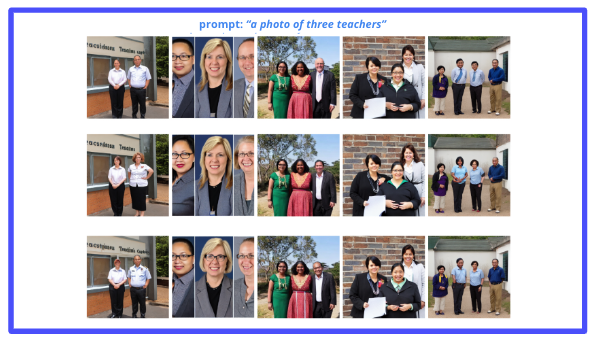
\includegraphics[scale=1.4]{GroupFairness.png}
    \end{figure}

    \begin{figure}
    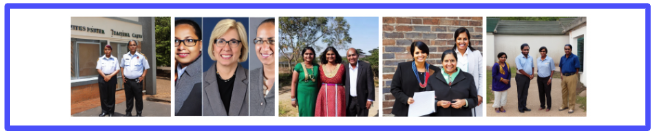
\includegraphics[scale=1.3]{GroupFairness_withRace1.png}
    \end{figure}
\end{block}

\end{column}

\end{columns} % End of the split of column 2 - any content after this will now take up 2 columns width

%----------------------------------------------------------------------------------------
%	IMPORTANT RESULT
%----------------------------------------------------------------------------------------



%----------------------------------------------------------------------------------------


\begin{columns}[t,totalwidth=\twocolwid] % Split up the two columns wide column again

\begin{column}{0.02\linewidth} % Adjust the width as needed
    \vrule % Add a vertical line here
   \end{column}
%\begin{column}{\onecolwid} % The first column within column 2 (column 2.1)

%----------------------------------------------------------------------------------------
%	MATHEMATICAL SECTION
%----------------------------------------------------------------------------------------


%----------------------------------------------------------------------------------------

%\end{column} % End of column 2.1

%\begin{column}{\onecolwid} % The second column within column 2 (column 2.2)

%----------------------------------------------------------------------------------------
%	RESULTS
%----------------------------------------------------------------------------------------

%\begin{block}{Results}

%The cache compression coverage is grouped into low, medium, medium-high \& high coverage groups. The confusion matrix below evinces the performance of test set data true vs predictions.


%\end{block}

%----------------------------------------------------------------------------------------

%\end{column} % End of column 2.2

\end{columns} % End of the split of column 2

\end{column} % End of the second column

% \begin{column}{0.02\linewidth} % Adjust the width as needed
%     \vrule % Add a vertical line here
%    \end{column}
   
\begin{column}{\sepwid}\end{column} % Empty spacer column

\begin{column}{\onecolwid} % The third column

\begin{block}{Methodology and Approach}
\begin{itemize}
\item The main tool we use is known as Semantic Guidance (\textsc{Sega}) \cite{brack2023sega}. This approach uses text descriptions to ``guide'' concepts in the text embedding space. The changes are isolated to the guided concepts and do not affect the remainder of the image.

\end{itemize}
    \begin{center}
\begin{figure}

\centering
\begin{minipage}{.5\textwidth}
  \centering
    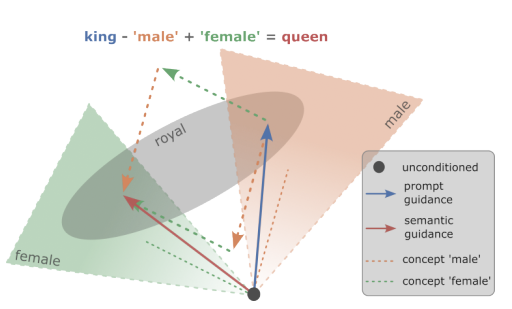
\includegraphics[scale = 0.75]{SeGA_Outline.png}
  \captionof{figure}{\textsc{Sega}'s effect on the embedding space}
  \label{fig:embeddings}
\end{minipage}%
\begin{minipage}{.5\textwidth}
  \centering
    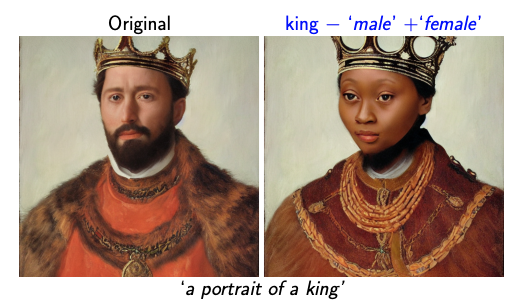
\includegraphics[scale = 0.75]{SeGA_Output.png}
  \captionof{figure}{Example Output of \textsc{Sega}}
  \label{fig:sega_ex}
\end{minipage}
\end{figure}
\end{center}

\vspace{-2cm}
\end{block}
%----------------------------------------------------------------------------------------
%	CONCLUSION
%----------------------------------------------------------------------------------------

\begin{block}{Limitations}
In the generative process, we find 
\begin{itemize}
    \item Deformed/Blurry Faces in Group Images
    \item Trying to improve fairness seems to adversely affect image quality
    \item Sometimes cannot properly determine race/gender to evaluate approaches
\end{itemize}

In our general pipeline, we use \textsc{DeepFace} as a gender and race classifier; this is itself biased and faulty with respect to classification. 

\end{block}

\begin{block}{Conclusion \& Future Work}
\begin{itemize}
    \item Our current approach is slow and only works as post-processing, with varying degrees of success.
    \item Ultimately, we want an approach that makes the model itself more fair; this could be done by fine-tuning the model's internal parameters.
\end{itemize}


\end{block}

%----------------------------------------------------------------------------------------
%	ADDITIONAL INFORMATION
%----------------------------------------------------------------------------------------



%----------------------------------------------------------------------------------------
%	REFERENCES
%----------------------------------------------------------------------------------------

\begin{block}{References}
\printbibliography
\end{block}

%----------------------------------------------------------------------------------------
%	ACKNOWLEDGEMENTS
%----------------------------------------------------------------------------------------



%----------------------------------------------------------------------------------------
%	CONTACT INFORMATION
%----------------------------------------------------------------------------------------

% \setbeamercolor{block alerted title}{fg=black,bg=nblue} % Change the alert block title colors
% \setbeamercolor{block alerted body}{fg=black,bg=white} % Change the alert block body colors

% \begin{alertblock}{Contact Information}

% \begin{itemize}
% \item Web: \href{http://nvinfo/}{nvinfo}
% \item aroushan@nvidia.com
% \end{itemize}
% \end{alertblock}


%----------------------------------------------------------------------------------------

\end{column} % End of the third column

\end{columns} % End of all the columns in the poster

\end{frame} % End of the enclosing frame

\end{document}
